\documentclass[UTF8, a4paper, 11pt]{article}
\usepackage{diagbox}
\usepackage{subfigure}
\usepackage[UTF8, scheme=plain]{ctex}
\usepackage{fontspec}
\usepackage{float}
\usepackage{amsmath}
\newtheorem{myDef}{Definition}
\usepackage{graphicx}
\usepackage{geometry}
\usepackage{listings}
\usepackage{xcolor}
\usepackage{caption}
\geometry{scale=0.8}
\linespread{1.5}
\usepackage{hyperref}
\usepackage{color}
\usepackage{fontspec}
\usepackage{enumitem}
\usepackage[linesnumbered,boxed]{algorithm2e}    
\usepackage{xeCJK}
\usepackage{indentfirst} 
\graphicspath{{Pics/}} 	% 在于.tex同级的目录下创建名为pic的文件夹,存放图片


\setlength{\parindent}{2em}

\lstset{
    language={python},
    frame=shadowbox,
    breaklines=true,
    numbers=left,
    backgroundcolor=\color[RGB]{245,245,244},
    rulesepcolor=\color{red!20!green!20!blue!20},
    numberstyle={\color[RGB]{0,192,192}\tiny},
    basicstyle=\footnotesize \fontspec{Source Code Pro}
}
\setenumerate[1]{itemsep=0pt,partopsep=0pt,parsep=\parskip,topsep=0pt}
\setitemize[1]{itemsep=0pt,partopsep=0pt,parsep=\parskip,topsep=0pt}
\setdescription{itemsep=0pt,partopsep=0pt,parsep=\parskip,topsep=0pt}


\title{	
\normalfont \normalsize
\textsc{School of Data and Computer Science, Sun Yat-sen University} \\ [25pt] %textsc small capital letters
\rule{\textwidth}{0.5pt} \\[0.4cm] % Thin top horizontal rule
\huge Random Forest\\ % The assignment title
\rule{\textwidth}{2pt} \\[0.5cm] % Thick bottom horizontal rule
\author{18308045 谷正阳}
\date{\normalsize\today}
}

\begin{document}
\maketitle
\tableofcontents
\newpage
\section{Importance function}
This function is used to evaluate how good a split of dataset is.
The basic idea is that if a label in each subset after a split dominates that subset, the split is good.
\subsection{Purity function}
To evaluate whether a label dominates a subset, we need to build a special function.
Since we do binary classification here, we just input the probability of one label in the subset into the function.
The return value should be high if the probability is close to 0 or 1.
Otherwise, the value should be low.
There are two common functions to evaluate the purity of a set, one of which is entropy, the other of which is negtive Gini index.
Entropy has the form of
\begin{equation}
	B(q)=-(q\log(q)+(1-q)\log(1-q)),
\end{equation}
while negtive Gini index has the form of
\begin{equation}
	Neg\_Gini(p)=-(1-(p^2+(1-p^2))).
\end{equation}
Based on these two purity functions, we build three importance functions.
\subsection{Information gain}
Information gain is to calculate the gain of entropy after the split.
It has the form of
\begin{equation}
	Gain(A)=B(\frac p{p+n})-\sum_{v=1}^V\frac{p_v+n_v}{p+n}B(\frac{p_v}{p_v+n_v}).
	\label{eq:gain}
\end{equation}
Because after the discretization every attributes' domains are binary, and $p,p+n$ are the same when comparing splits, the actual equation used here is
\begin{equation}
	Neg\_Remainder\_Mul\_N(A)=(p_0+n_0)(-B(\frac{p_0}{p_0+n_0}))+(p_1+n_1)(-B(\frac{p_1}{p_1+n_1})).
\end{equation}
The function NEG\_REMAINDER\_MUL\_N below takes all the features as inputs and returns an array containing all their $Neg\_Remainder\_Mul\_N$.
\begin{lstlisting}
def NEG_B(q):
    I_q = 1 - q
    return xlogy(q, q) + xlogy(I_q, I_q)

def NEG_REMAINDER_MUL_N(S, F):
    label = S[:, -1:]
    S1 = S[:, F]

    p1 = np.sum(S1 & label)
    N1 = np.sum(S1)

    p0 = np.sum(label) - p1
    N0 = S.shape[0] - N1

    return N1 * NEG_B(p1 / N1) + N0 * NEG_B(p0 / N0)
\end{lstlisting}
\subsection{Information gain ratio}
The information gain\ref{eq:gain} has a weakness, which is that if the domain of an attribute is too big, the second term $\sum_{v=1}^V\frac{p_v+n_v}{p+n}B(\frac{p_v}{p_v+n_v})$ can be really small.
Therefore, the information gain prefer those attributes with larger dommain.
The information gain ratio has the form of
\begin{equation}
	Gain\_ratio(A)=\frac{Gain(A)}{-\sum_{v=1}^V\frac{p_v+n_v}{p+n}\log(\frac{p_v+n_v}{p+n})},
\end{equation}
which is actually add a penalty on the information gain\ref{eq:gain}.
If the domain of an attribute is large, the $-\sum_{v=1}^V\frac{p_v+n_v}{p+n}\log(\frac{p_v+n_v}{p+n})$ will be large, so its gain ratio is small.

However, since all the attributes here have binary domains, the information gain ratio is the same as the information gain.
\subsection{Negative Gini gain}
This has a similar form as the information gain\ref{eq:gain}, since it's actually replace the $\log(p)$ with its approximate substitution $p-1$.
This can be calculated faster than information gain since $p-1$ is easier to calculate than $\log(p)$.
\begin{lstlisting}
def NEG_GINI_MINUS_1(p):
    return p ** 2 + (1 - p) ** 2

def NEG_GINI_INDEX_MINUS_1_MUL_N(S, F):
    label = S[:, -1:]
    S1 = S[:, F]

    p1 = np.sum(S1 & label)
    N1 = np.sum(S1)

    p0 = np.sum(label) - p1
    N0 = S.shape[0] - N1

    return N1 * NEG_GINI_MINUS_1(p1 / N1) + N0 * NEG_GINI_MINUS_1(p0 / N0)
\end{lstlisting}
\section{Discretization}
Since the data preprocessed in the last part of project are all continuous value.
And the decision tree requires those attributes to be discretized.
This part is implemented in function read.
The function is used to find the best split point to split the domain of an attribute into 2 labels.
\subsection{The first step: to calculate all split points}
To discretize an attibute, firstly, we build an array containing all values appear in the attribute.
And we sort it and remove all the duplicate values in it.
Now we get a sorted domain of the attributes.
Then we can use matrix operation to generate an array containing all split points.
\begin{lstlisting}
mids = X[:, f]
np.sort(mids)
mids = np.unique(mids)
mids = (mids[:-1] + mids[1:]) / 2
\end{lstlisting}
\subsection{The second step: to choose the best split point}
We can get scores of split points using importance function defined above. and choose the split with highest importance.
\begin{lstlisting}
x_best = None
mid_best = None
score_best = -float("inf")
for mid in mids:
    x = (X[:, f:f + 1] >= mid)
    score = IMPORTANCE(np.concatenate((x, Y), axis=1), np.array([0]))
    if score_best < score:
    x_best = x
    mid_best = mid
    score_best = score
X[:, f:f + 1] = x_best
threshold[f] = mid_best
\end{lstlisting}
\subsection{Comparison between Numpy version and PyTorch version}
Since there are some matrix operation, it seems like the calculation can be speeded up by CUDA which is supported by PyTorch but not supported by NumPy.
Therefore, I implement discretization in 2 versions and compare their performance.
\begin{figure}[H]
    \centering
    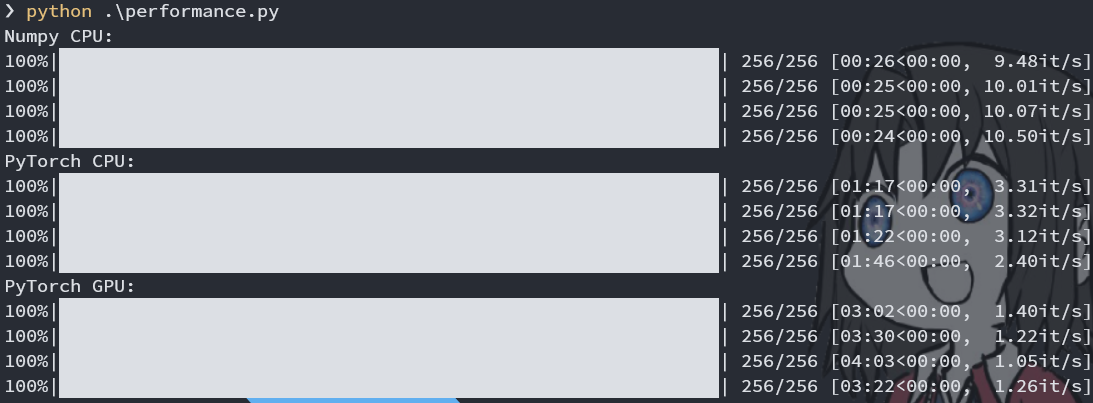
\includegraphics[width=0.8\textwidth]{CPU_GPU.png}
\end{figure}
The result shows that neither PyTorch with CPU nor PyTorch with GPU is faster than Numpy.
The reason may be that there are lots of loop operation which performs worse on PyTorch than on Numpy.
\section{Experiment}
I divide the output into 4 outputs like what I do in the last project.
Therefore I need to build 4 random forests in each model.
\subsection{Different importance functions}
I test different importance functions.
Since we have discussed that information gain ratio and information gain are the same before, we just test the performance of information gain and negative Gini index gain.
\begin{figure}[H]
    \centering
    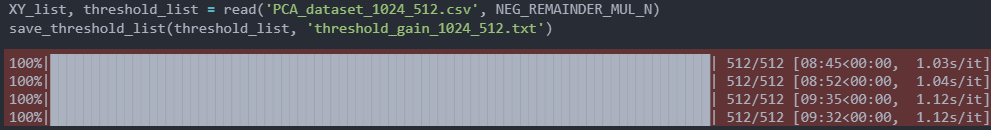
\includegraphics[width=0.8\textwidth]{1024_512_gain_thre.png}
    \caption{Discretization using information gain}
\end{figure}
\begin{figure}[H]
    \centering
    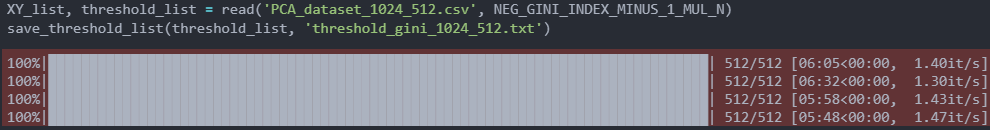
\includegraphics[width=0.8\textwidth]{1024_512_gini_thre.png}
    \caption{Discretization using negative Gini index gain}
\end{figure}
\begin{figure}[H]
    \centering
    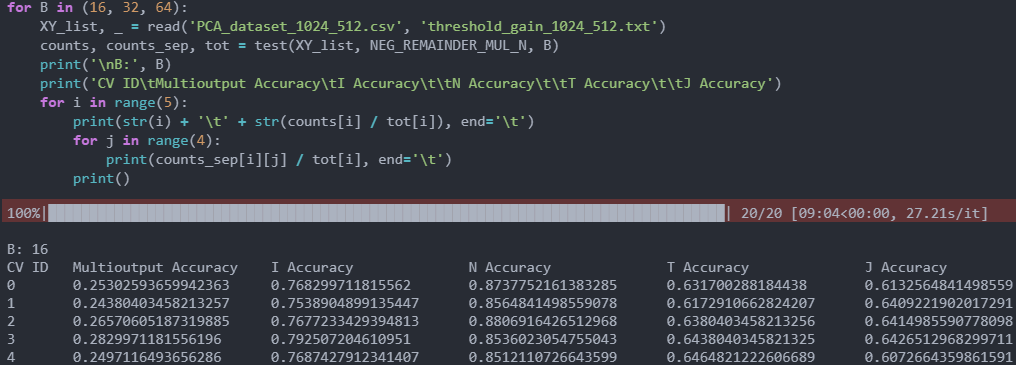
\includegraphics[width=0.8\textwidth]{1024_512_16_gain.png}
    \caption{Attributes selection using information gain}
\end{figure}
\begin{figure}[H]
    \centering
    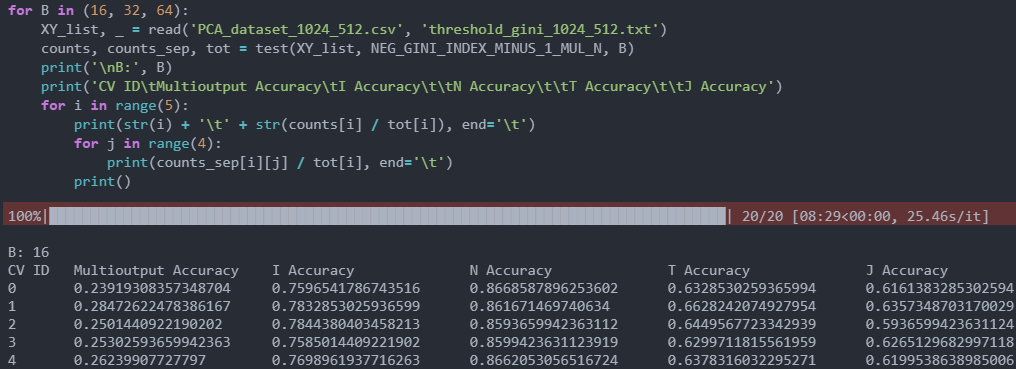
\includegraphics[width=0.8\textwidth]{1024_512_16_gini.png}
    \caption{Attributes selection using negative Gini index gain}
\end{figure}
Their accuracy is almost the same and the time consumption of Gini is a little less than that of gain.
\subsection{Different types of features}
I test several kinds of features as follows.
\begin{figure}[H]
    \centering
    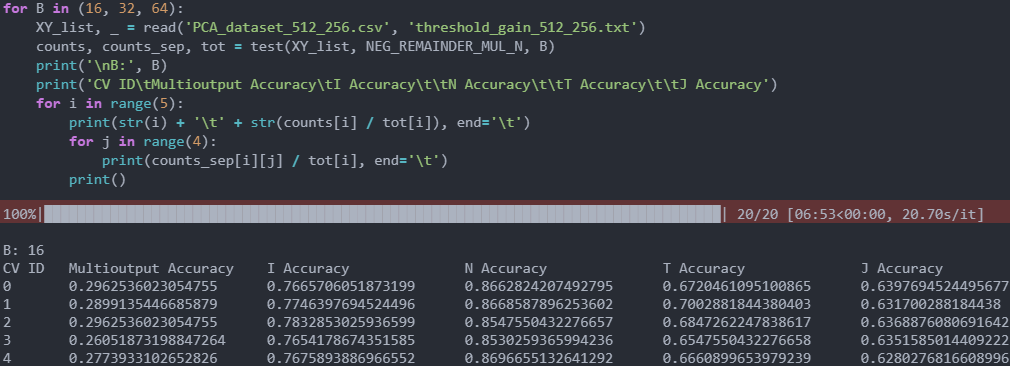
\includegraphics[width=0.8\textwidth]{512_256_16_gain.png}
    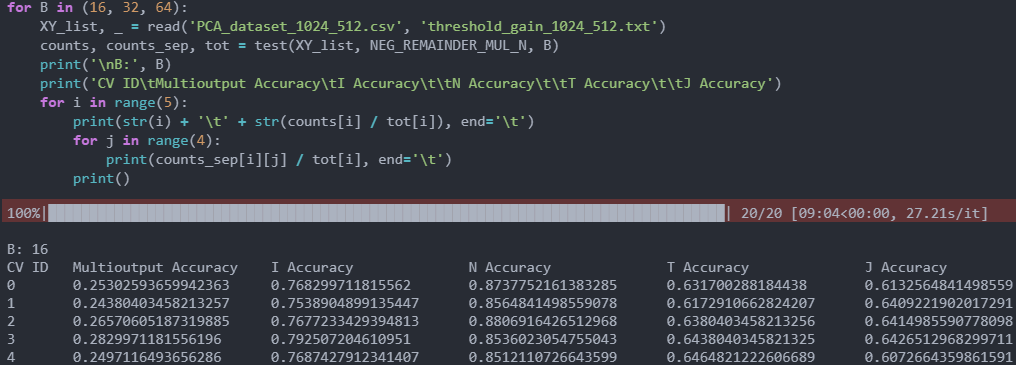
\includegraphics[width=0.8\textwidth]{1024_512_16_gain.png}
    \caption{Tf-Idf processed by feature selection and PCA}
\end{figure}
\begin{figure}[H]
    \centering
    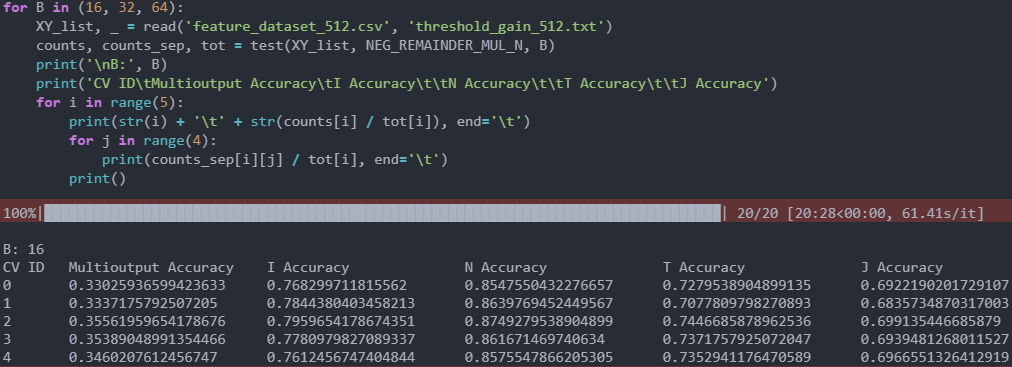
\includegraphics[width=0.8\textwidth]{512_16_gain.png}
    \caption{Tf-Idf processed by feature selection}
\end{figure}
\begin{figure}[H]
    \centering
    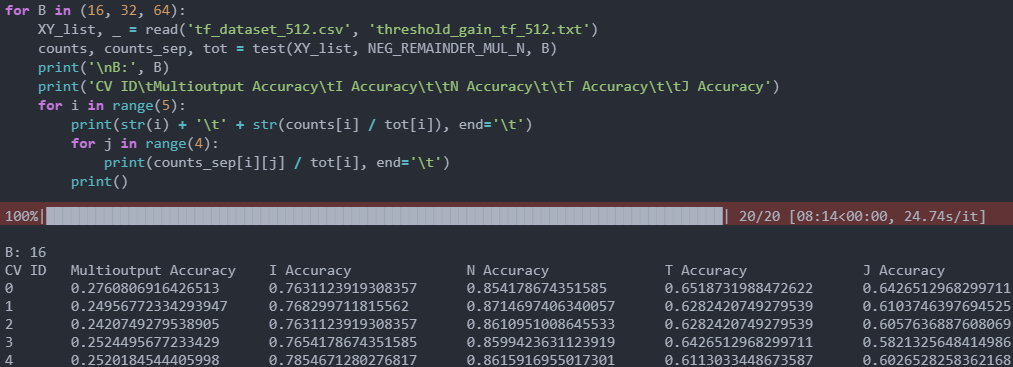
\includegraphics[width=0.8\textwidth]{tf_512_16_gain.png}
    \caption{Tf processed by feature selection}
\end{figure}
It turns out that TF-Idf processed by feature selection has the best performance.
\subsection{Different number of features}
It seems like the larger the number of features is, the better the decision tree predicts.
However, if the number of features is too large, those trival features may greatly affect the random forest.
That is because the random forest needs to randomly select attributes before choosing the best attribute.
Too many trival features may cause that the features randomly selected are all trival.
\begin{figure}[H]
    \centering
    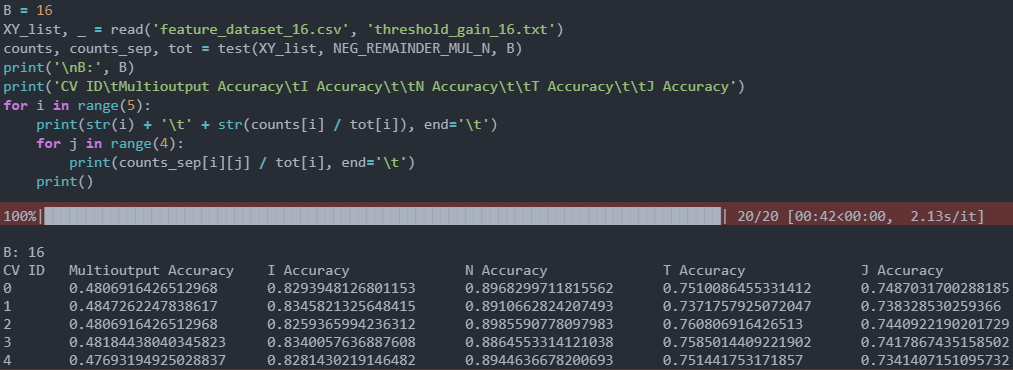
\includegraphics[width=0.8\textwidth]{16_16_gain.png}
    \caption{16 features}
\end{figure}
\begin{figure}[H]
    \centering
    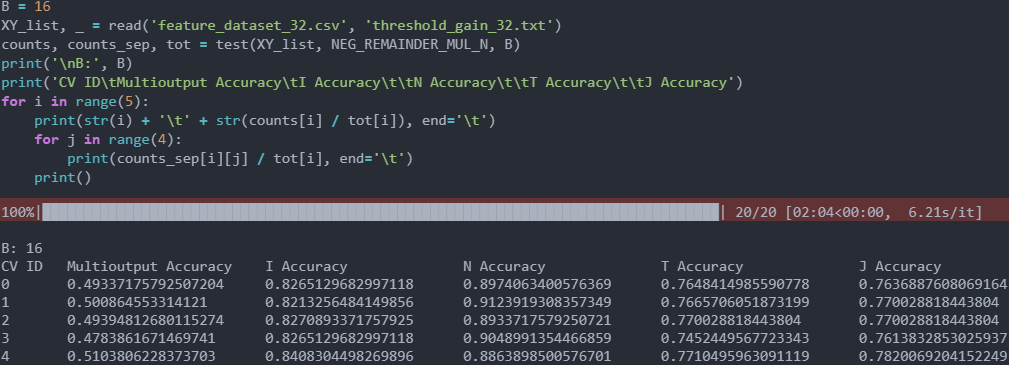
\includegraphics[width=0.8\textwidth]{32_16_gain.png}
    \caption{32 features}
\end{figure}
\begin{figure}[H]
    \centering
    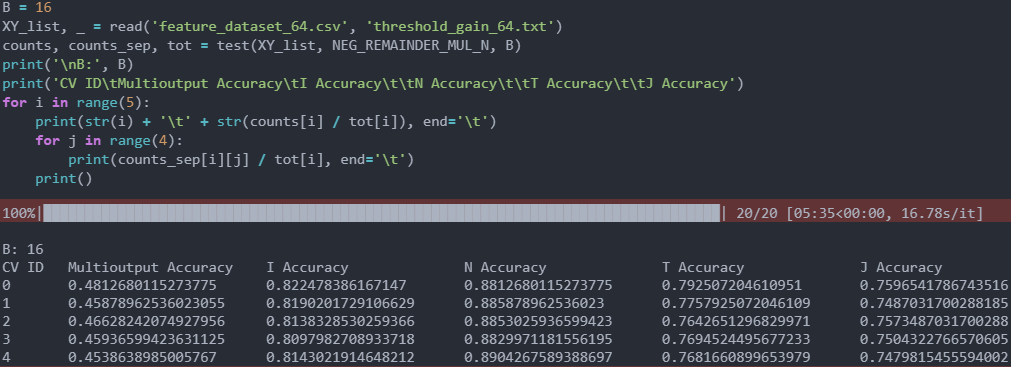
\includegraphics[width=0.8\textwidth]{64_16_gain.png}
    \caption{64 features}
\end{figure}
\begin{figure}[H]
    \centering
    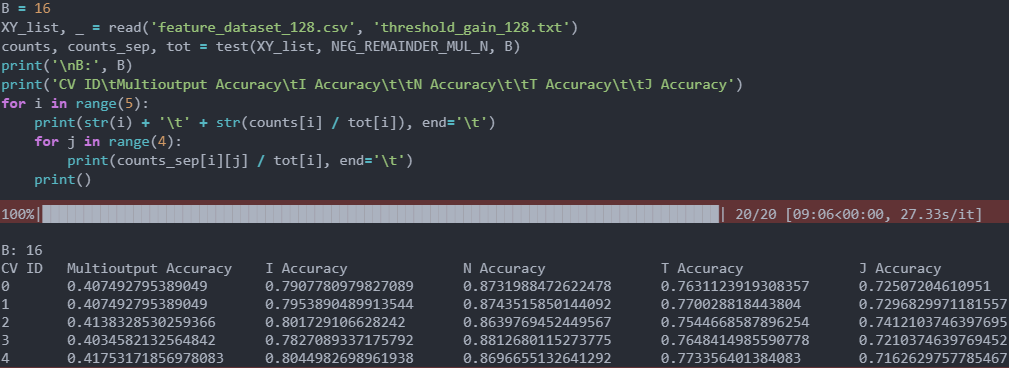
\includegraphics[width=0.8\textwidth]{128_16_gain.png}
    \caption{128 features}
\end{figure}
\begin{figure}[H]
    \centering
    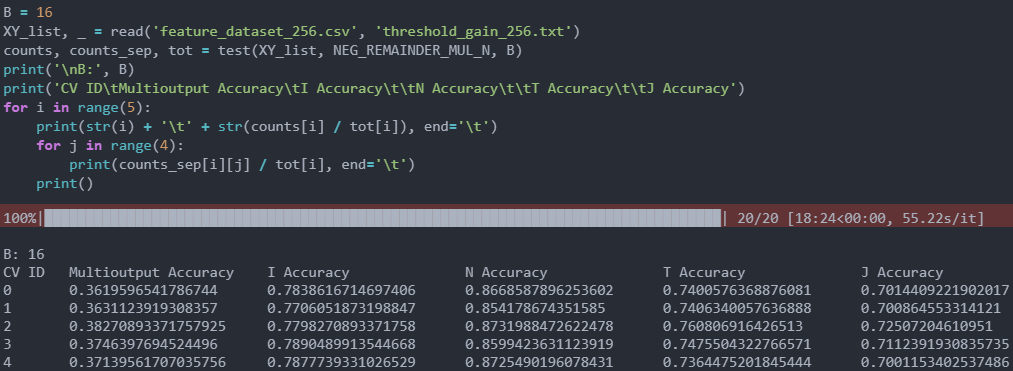
\includegraphics[width=0.8\textwidth]{256_16_gain.png}
    \caption{256 features}
\end{figure}
\begin{figure}[H]
    \centering
    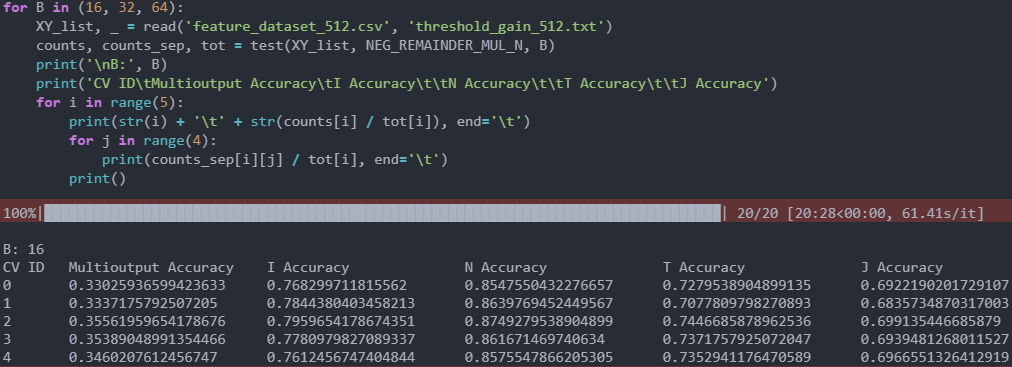
\includegraphics[width=0.8\textwidth]{512_16_gain.png}
    \caption{512 features}
\end{figure}
\begin{figure}[H]
    \centering
    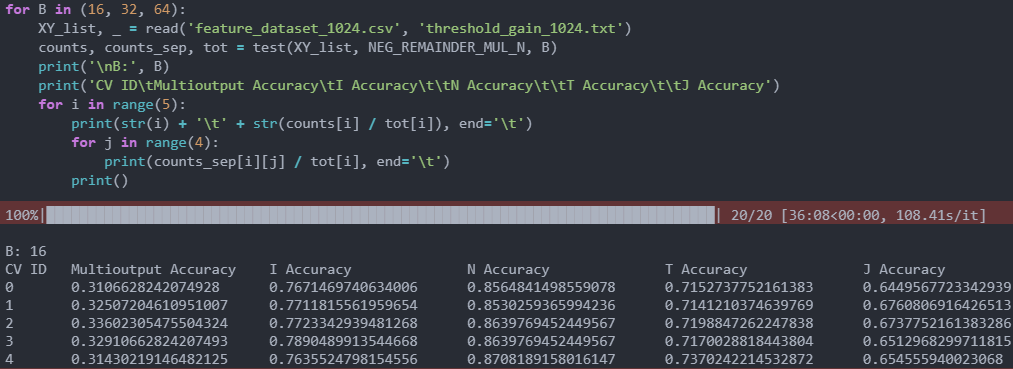
\includegraphics[width=0.8\textwidth]{1024_16_gain.png}
    \caption{1024 features}
\end{figure}
The random forest with 32 features have the best performance.
\subsection{Different number of trees in a forest}
\begin{figure}[H]
    \centering
    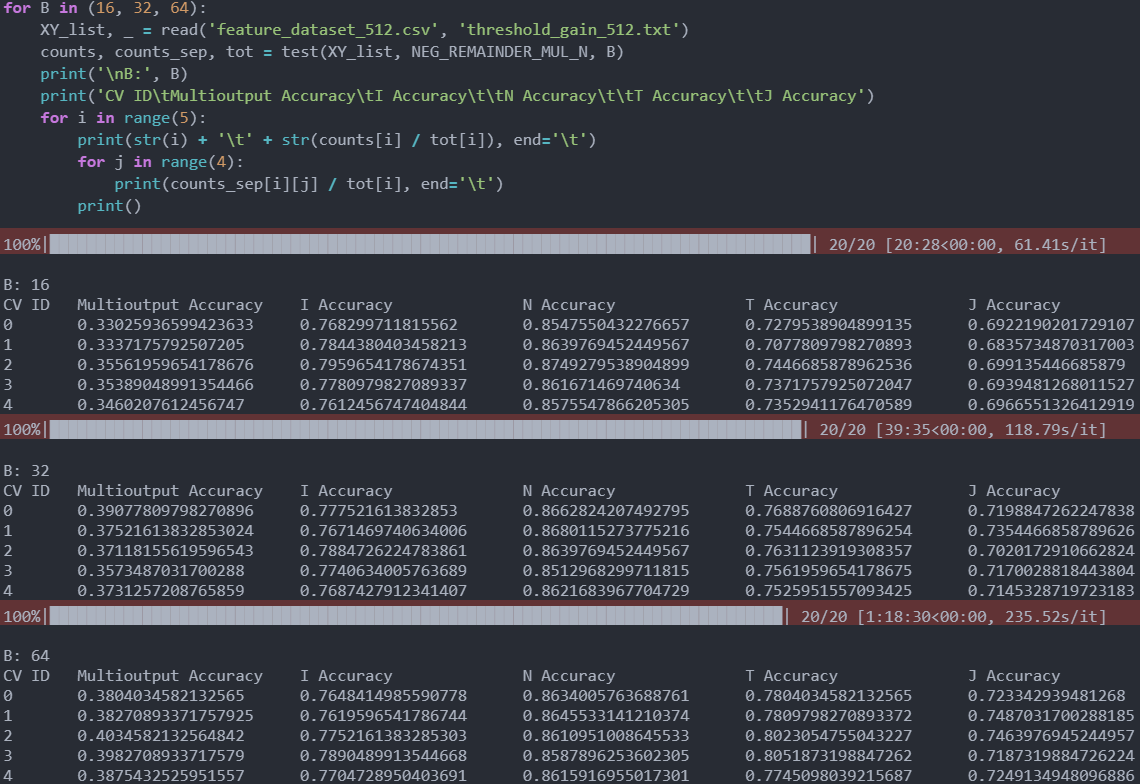
\includegraphics[width=0.8\textwidth]{512_gain.png}
    \caption{512 features}
\end{figure}
\begin{figure}[H]
    \centering
    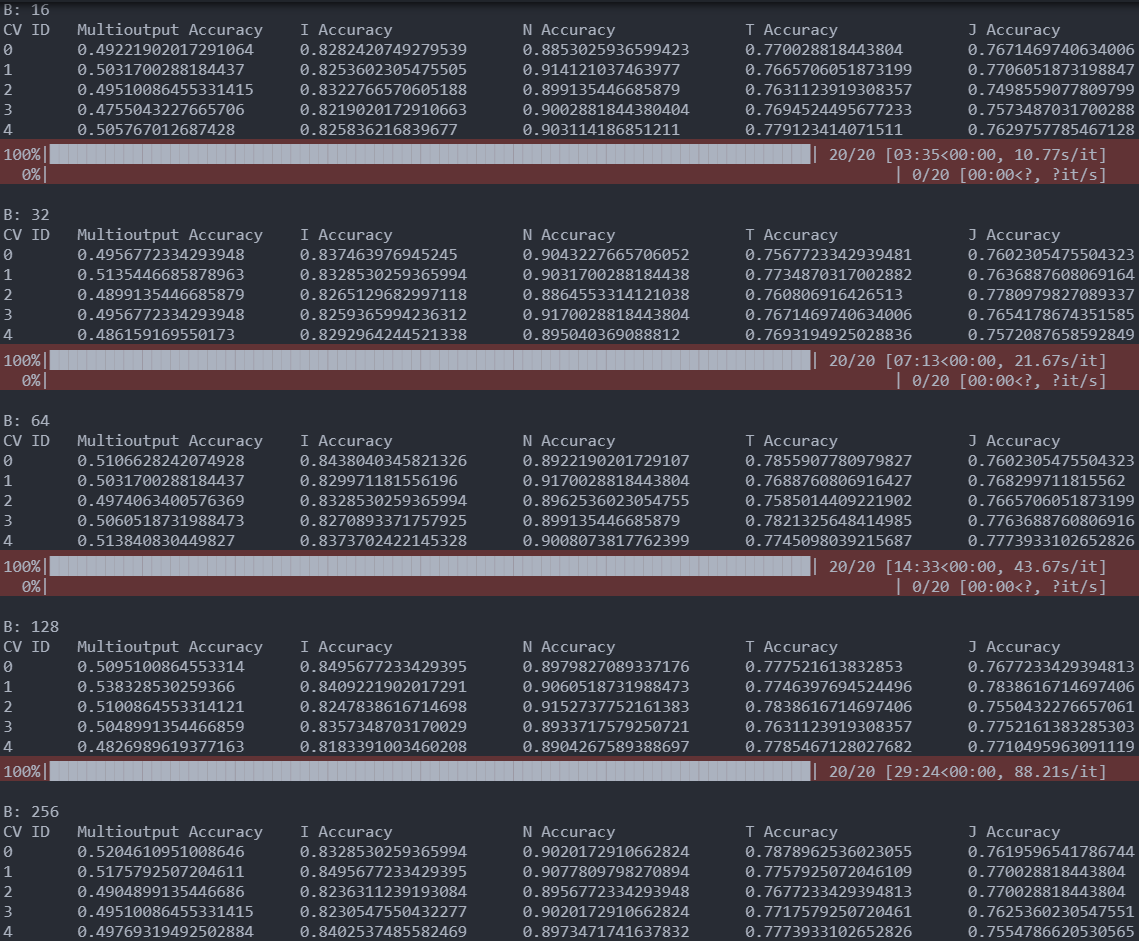
\includegraphics[width=0.8\textwidth]{32_gini.png}
    \caption{32 features}
\end{figure}
When the number of features is large, the influence of the number of trees is big.
When the number of features is little, the influence of the number of trees is small.
It seems like the model falls into a locally optimal solution.
And this also support for the explanation of why large number of features can have bad result.
Large number of trees can cover the influence caused by frequently selection of trival attributes.
\section{Conclusions}
The result is not good enough compared with SVM.
Reasons may be that the model falls into a locally optimal solution, or these types of features may be bad for random forest, or the binary discretization is not good enough.
%\clearpage
%\bibliography{E:/Papers/LiuLab}
%\bibliographystyle{apalike}
\end{document}
%%% Local Variables:
%%% mode: latex
%%% TeX-master: t
%%% End:
